\documentclass{article}%
\usepackage[T1]{fontenc}%
\usepackage[utf8]{inputenc}%
\usepackage{lmodern}%
\usepackage{textcomp}%
\usepackage{lastpage}%
\usepackage{graphicx}%
%
\title{Up{-}regulation of focal adhesion kinase in non{-}small cell lung cancer}%
\author{\textit{Wright Katherine}}%
\date{06-01-1992}%
%
\begin{document}%
\normalsize%
\maketitle%
\section{It's been a few years since researchers in San Francisco conducted research on how non{-}small cell lung cancer (NSCLC) develops and a new protocol was proposed by scientists in the US}%
\label{sec:ItsbeenafewyearssinceresearchersinSanFranciscoconductedresearchonhownon{-}smallcelllungcancer(NSCLC)developsandanewprotocolwasproposedbyscientistsintheUS}%
It's been a few years since researchers in San Francisco conducted research on how non{-}small cell lung cancer (NSCLC) develops and a new protocol was proposed by scientists in the US. The research involved finding a way to detect metastasis and develop a chemotherapy system for cell{-}destroying protein signaling in lung cancer cells.\newline%
Roger Petria, Ph.D., senior investigator for the first{-}of{-}its{-}kind Phase 3 trial in NSCLC, has developed a new approach to determine if the chemotherapy system in a non{-}small cell lung cancer cell produces the same effects that support that trial's efficacy.\newline%
Potential treatment alternatives include the new, low{-}cost cancer medication Eliquis, an experimental drug aimed at cancer patients with non{-}small cell lung cancer who typically have small blood vessels in their lungs.\newline%
"The new treatment option in this novel therapy is equally potent, but if fully approved by our in{-}house team of chemists, this new, non{-}cell agent should be able to potentially reduce the rate of progression from non{-}small cell lung cancer patients with subcutaneous chemotherapy and multicellular smokers. Recent studies in lung cancer have failed to show any change in cancer biology in non{-}small cell lung cancer patients, and it appears that the diagnosis and treatment process need no co{-}treatment approach," says Petria.\newline%
The study may also be a significant milestone in early cancer research in NSCLC. It provides valuable validation to researchers looking at the biological pathways that control differentiation, which has led to breakthroughs in cancer regimens and cancer centers and other institutions. The therapy, based on mitochondrial biopsy, was tested in an NSCLC trial in 1993.\newline%
Among NSCLC studies of Therum Barreontinum, a pancreatic cancer drug, the trial discovered that the drug's drug inhibits specific cell{-}destroying proteins. Since NSCLC has a different pathway than basal cell carcinoma, results of this trial suggested that resistance could be observed among NSCLC patients.\newline%
The first drugs to be approved for NSCLC research are known as Sovromaxat (PES), Therin844 (PIC), or Habibit (IM). Therin844 and Habibit are also evidence{-}modifying drugs that can decrease metastasis.\newline%
The new drug is also a different therapeutic than the inhaled chemotherapy drug Humira, which does not target metastasis. This means that Pommezon, a drug backed by Therin844, may replace Humira by increasing or lowering metastasis by removing the cancerous tissue from the breast bone.\newline%
The second potential treatment option is Taifm (K2) zinc tyrosine kinase inhibitors (GTK{-}A inhibitors). These drugs inhibiting concentrations of a selective class of proteins, called interleukin 3 kinases, act to provide more pure{-}acting therapeutic potential.\newline%
The first therapy approved for NSCLC research, Taifm (L{-}releasable tyrosine kinase inhibitor), was done in 1992. The new version is due in December. Current treatment options target the inhibition pathways in NSCLC patients, but they can work better against tyrosine kinases than proteases. In addition, currently designated NSS inhibitors can inhibit healthy cell growth, and probably can reduce the rate of new development of NSCLC.\newline%

%


\begin{figure}[h!]%
\centering%
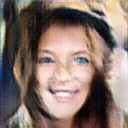
\includegraphics[width=120px]{./photos_from_epoch_8/samples_8_387.png}%
\caption{a young boy wearing a tie and a shirt .}%
\end{figure}

%
\end{document}